\begin{pregunta}
\puntaje{5}
\begin{cuerpo}
La im\'agen
\begin{center}
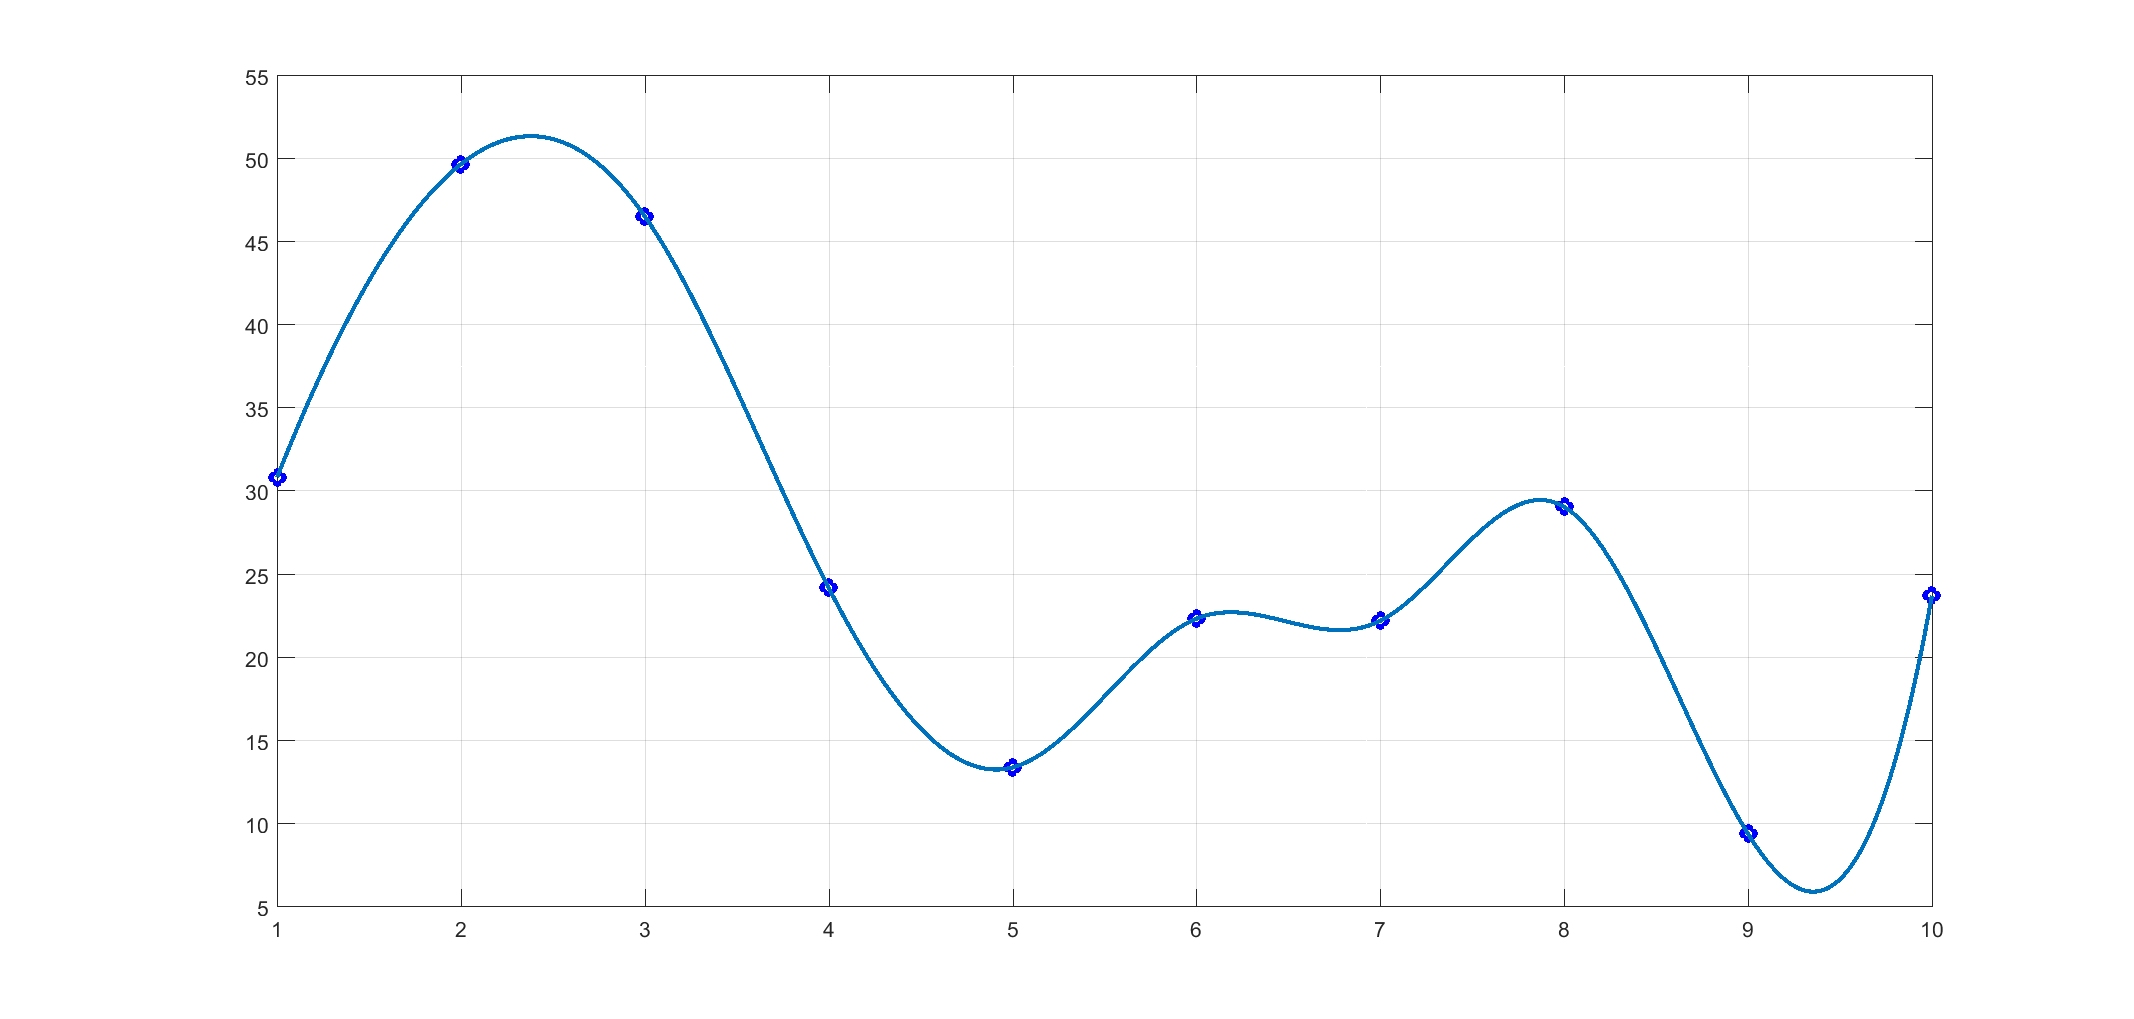
\includegraphics[width=0.8\textwidth]{./img/p24.jpg}
\end{center}
muestra la funci\'on de interpolaci\'on de una colecci\'on de puntos generada mediante
\end{cuerpo}

\begin{alternativas}
{un spline.}
{un polinomio interpolante de grado 9}
{un polinomio interpolante de grado 10}
{un polinomio interpolante de grado 8}
\end{alternativas}
\justificacion{0cm}
\end{pregunta}